\documentclass[12pt, a4paper]{article}

\usepackage[left=3cm, top=3cm, text={15cm,23.5cm}]{geometry}
\usepackage[T1]{fontenc} 
\usepackage[bf]{caption}
\usepackage{hyperref}
\usepackage[all]{hypcap}
\usepackage[utf8]{inputenc}
\usepackage{graphicx}
\usepackage[slovak, english]{babel}
\selectlanguage{slovak}
\usepackage{subfig}
\usepackage{color}
\usepackage{url}
\inputencoding{utf8}
\usepackage{hyperref}
\usepackage[all]{hypcap}
\hypersetup{colorlinks=false, linkbordercolor=1 1 1, citebordercolor=1 1 1}
\usepackage{amsmath}

\usepackage[ruled,vlined,czech,linesnumbered]{algorithm2e}
\providecommand{\dontprintsemicolon}{\DontPrintSemicolon}

\providecommand{\uv}[1]{\quotedblbase #1\textquotedblleft}

\title{Automatická kalibrácia RGB kamery a LiDARu\\Velodyne pomocou evolučnej stratégie}
\author{Martin Veľas\\ivelas@fit.vutbr.cz}
\date{\today}


%--------------------------------------------------------------------------------


\begin{document}
\selectlanguage{slovak}
\maketitle
%\linenumbers

%%%%%%%%%%%%%%%%%%%%%%%%%%%%%%%%%%%%%%%%%%%%%%%%%%%%%%%%%%%%%%%%%%%%%%%%%%%%%%%%
\section{Úvod}

Fúzia výstupov viacerých senzorov ponúka možnosť získať bohatší informačný obsah, ktorý samostatným senzorickým dátam chýba. Môže ísť napríklad o spojenie snímkov viacerých diagnostických prístrojov v medicíne\cite{jan} alebo spojenie $3$D mračna bodov \emph{LiDARu} so snímkom \emph{kamery}, o ktorom pojednáva táto práca.

\begin{figure}[h!]
	\center
	\subfloat[Obrázok kamery]{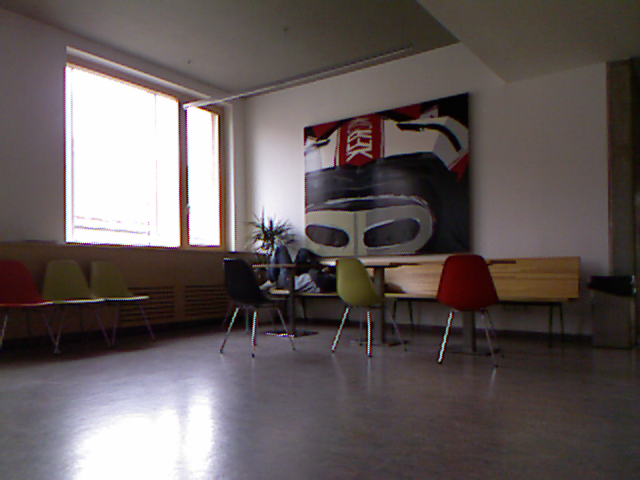
\includegraphics[height=0.23\textwidth]{fig/camera_image.png}}
	\quad
	\subfloat[Mračno LiDARu Velodyne]{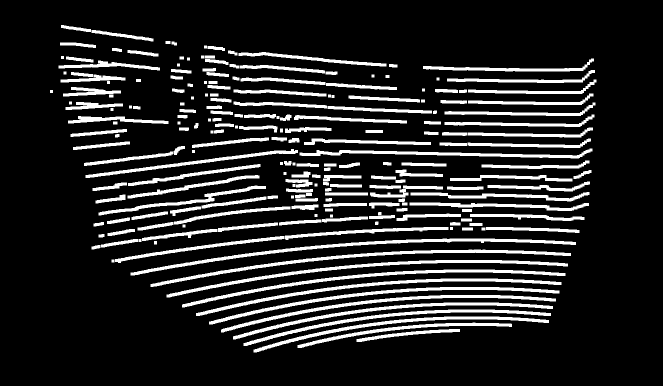
\includegraphics[height=0.23\textwidth]{fig/gray_cloud.png}}
	\quad
	\subfloat[Ofarbené mračno]{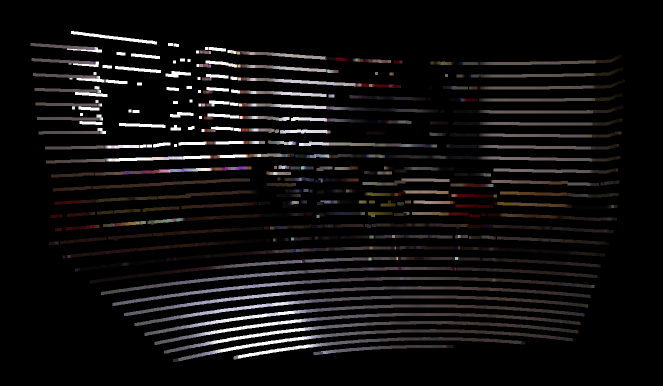
\includegraphics[height=0.25\textwidth]{fig/colored_cloud.png}}
\caption{Snímok RGB kamery, mračno bodov ako výstup LiDARu Velodyne a ofarbené mračno bodov na získané fúziou uvedených senzorických dát na základe kalibrácie LiDARu s kamerou.\cite{taylor}\label{fig:color-cloud}}
\end{figure}

Lidar (laserový radar) poskytuje relatívne presnú informáciu o polohe objektov v priestore vo forme mračna bodov. Oproti tomu kamera zachytáva informáciu o farebných vlastnostiach povrchu objektov. Fúziou uvedených senzorov môžeme získať napríklad zafarbené mračno bodov pre bohatšie zobrazenie scény -- viď. obr. \ref{fig:color-cloud}.

Ďalším využitím takto spojených senzorov je možnosť priradenia obrazových lokálnych príznakov k jednotlivým bodom mračna. Tieto príznaky sú ďalej použité pre potreby lokalizácie robota v priestore či detekcii zmien v scéne.



%%%%%%%%%%%%%%%%%%%%%%%%%%%%%%%%%%%%%%%%%%%%%%%%%%%%%%%%%%%%%%%%%%%%%%%%%%%%%%%%
\section{Popis senzorov}
V tejto kapitole budú popísané senzory použité pre fúziu -- teda kamera a lidar. Keďže pri spomínanej fúzii ide o dodanie farebnej informácie do mračna bodov, je využitá klasická RGB kamera senzoru Kinect, pričom hĺbková mapa, ktorá je taktiež jeho výstupom nie je využitá. Netradičnejším a teda aj zaujímavejším senzorom pre popis je laserový radar Velodyne. 

Oba uvedené senzory sú inštalované na našej robotickej platforme (obr. \ref{fig:velodyne}), ktorá využíva robotický operačný systém \emph{ROS} pre unifikovanú prácu so senzorickými dátami pomocou systému \emph{topic-ov}, riešenie závislostí, konfiguráciu a komunikáciu aplikácií.

\subsection{Velodyne lidar}

Velodyne je lidar s vysokým rozlíšením, ktorý je vyrábaný firmou s rovnomenným názvom\cite{velodyne}. Samotný senzor spoločne s príkladom jeho výstupu je znázornený na obrázku \ref{fig:velodyne}. Senzor sa otáča rýchlosťou $10$Hz za sekundu a sníma scénu v rozsahu $360^{\circ}$ okolo senzoru. Prichádza v dvoch základných prevedeniach -- s $32$ a $64$ laserovými lúčmi, z čoho vychádza počet zosnímaných prstencov a teda aj miera podrobnosti získaného mračna bodov.

\begin{figure}[h]
\center
	\subfloat[Velodyne]{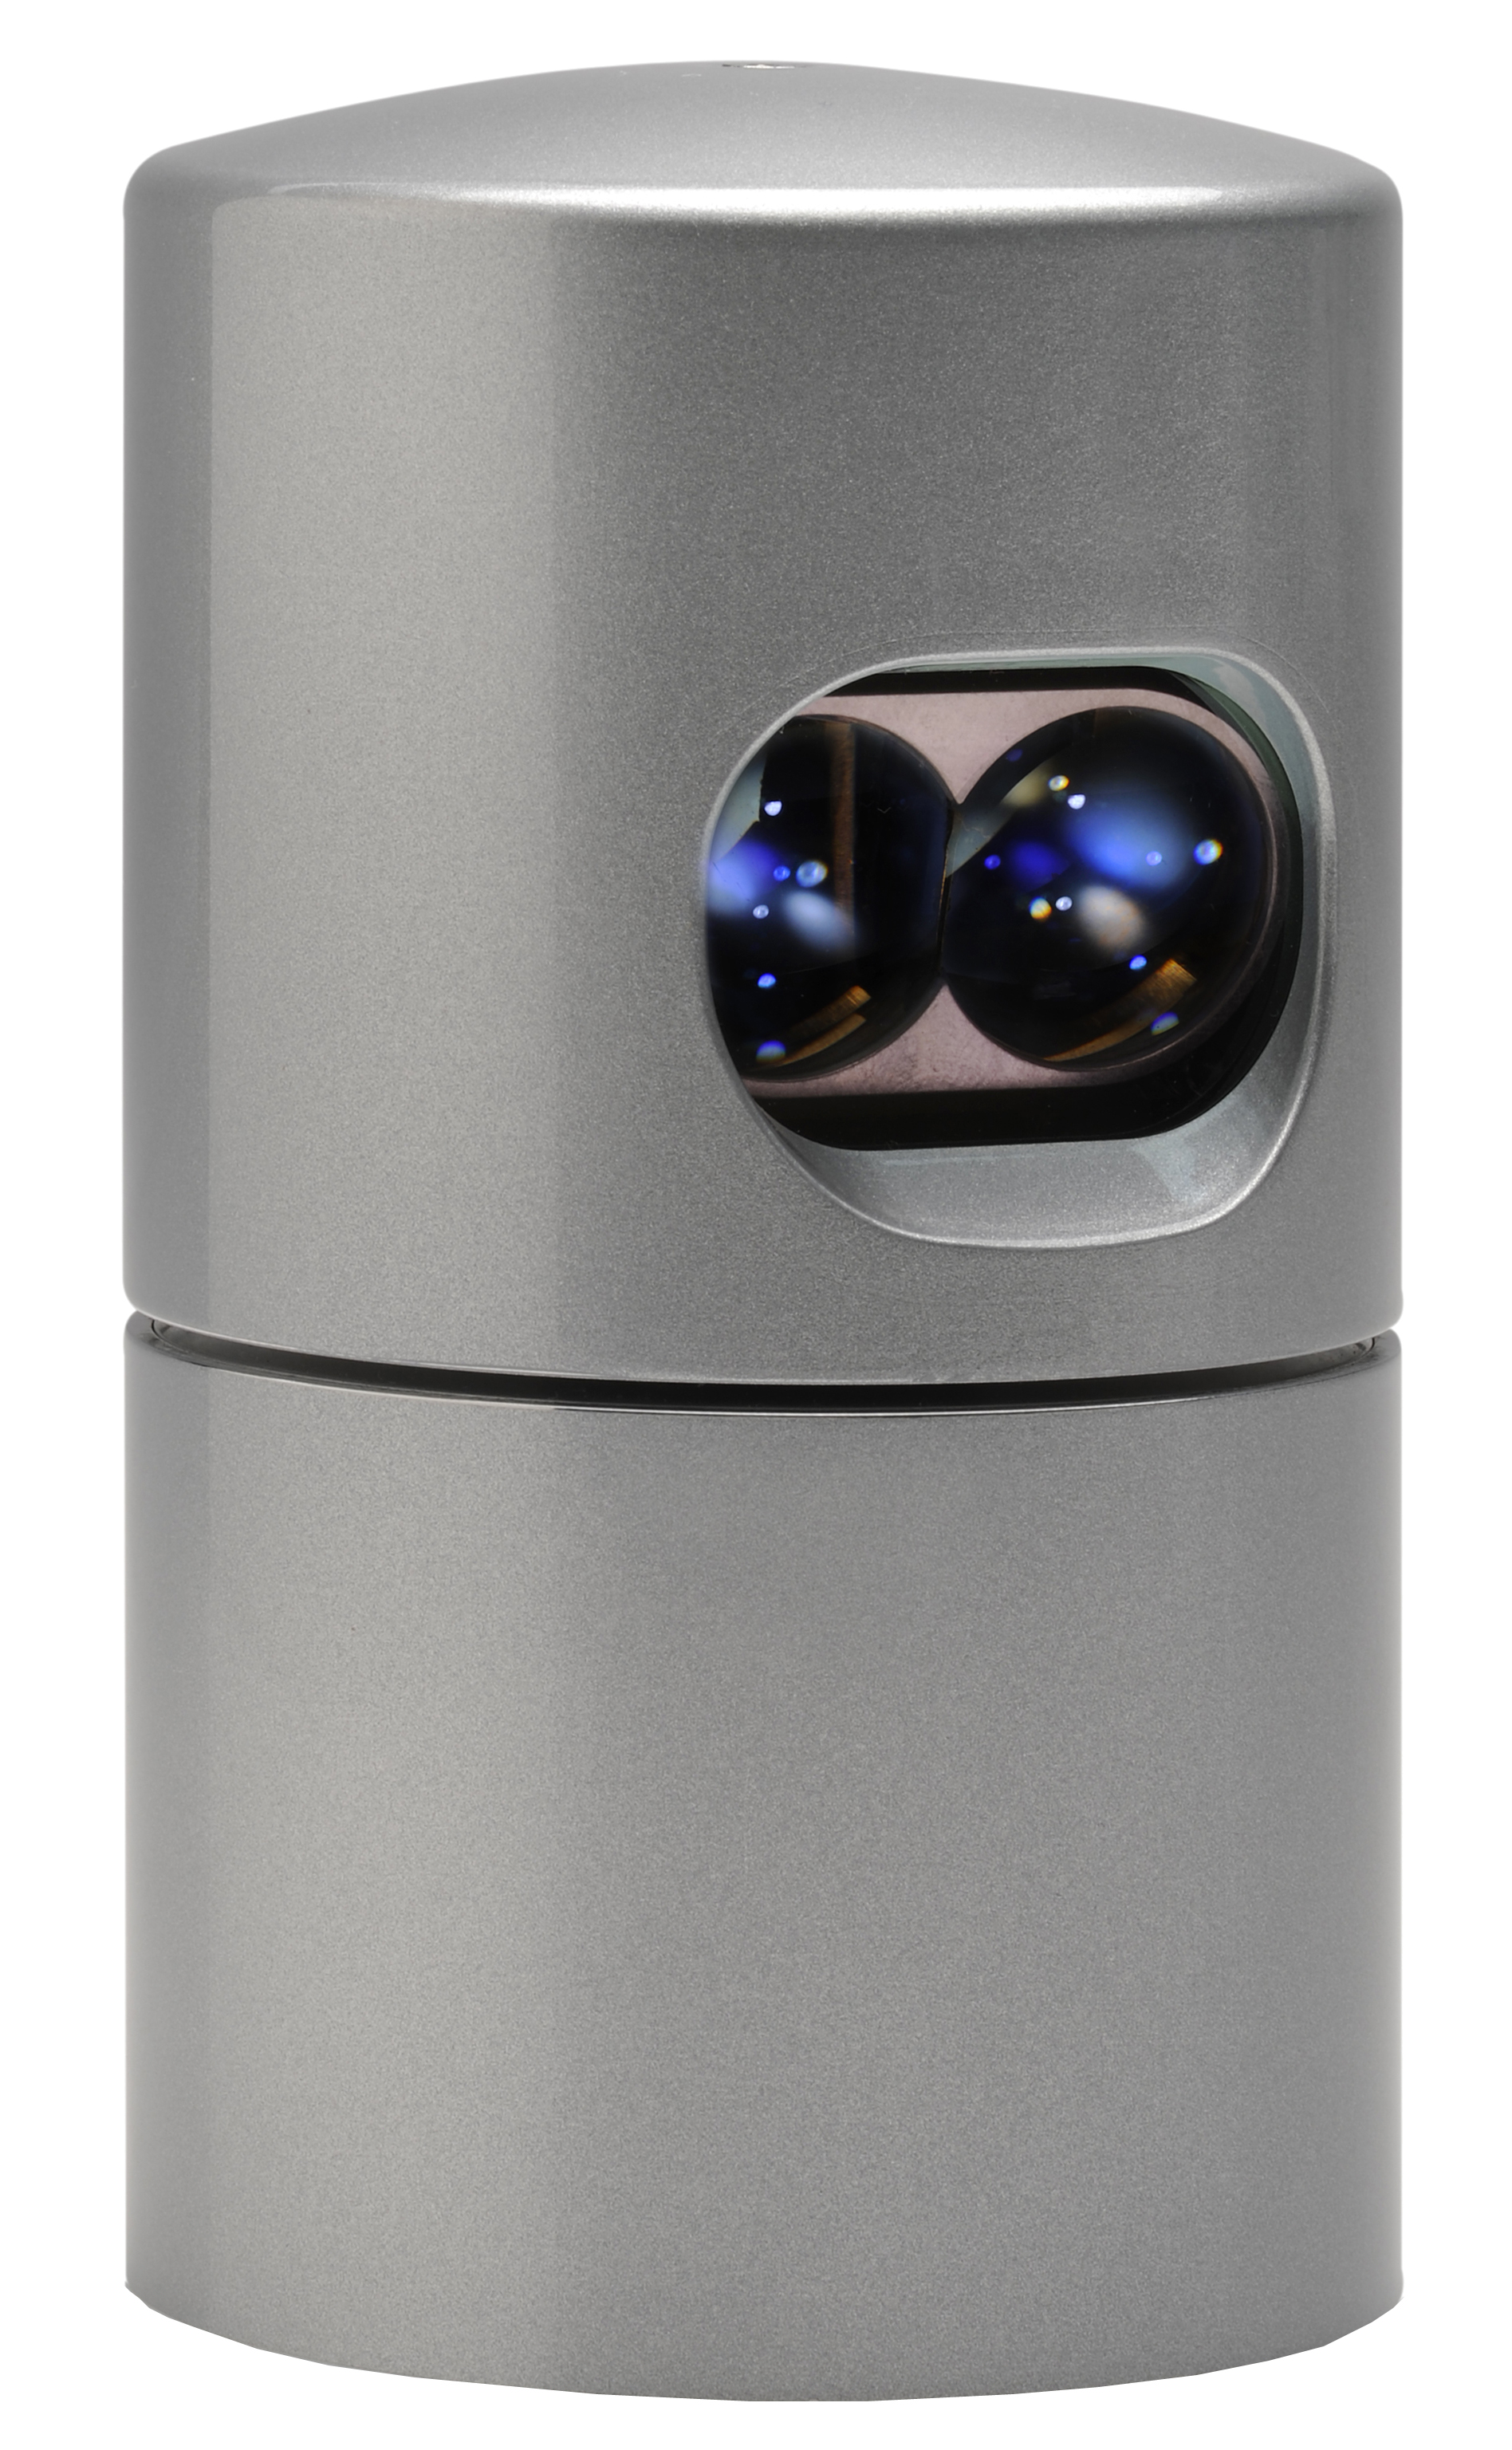
\includegraphics[height=0.32\textwidth]{fig/velodyne_32.png}}
	\quad
	\subfloat[Príklad výstupu]{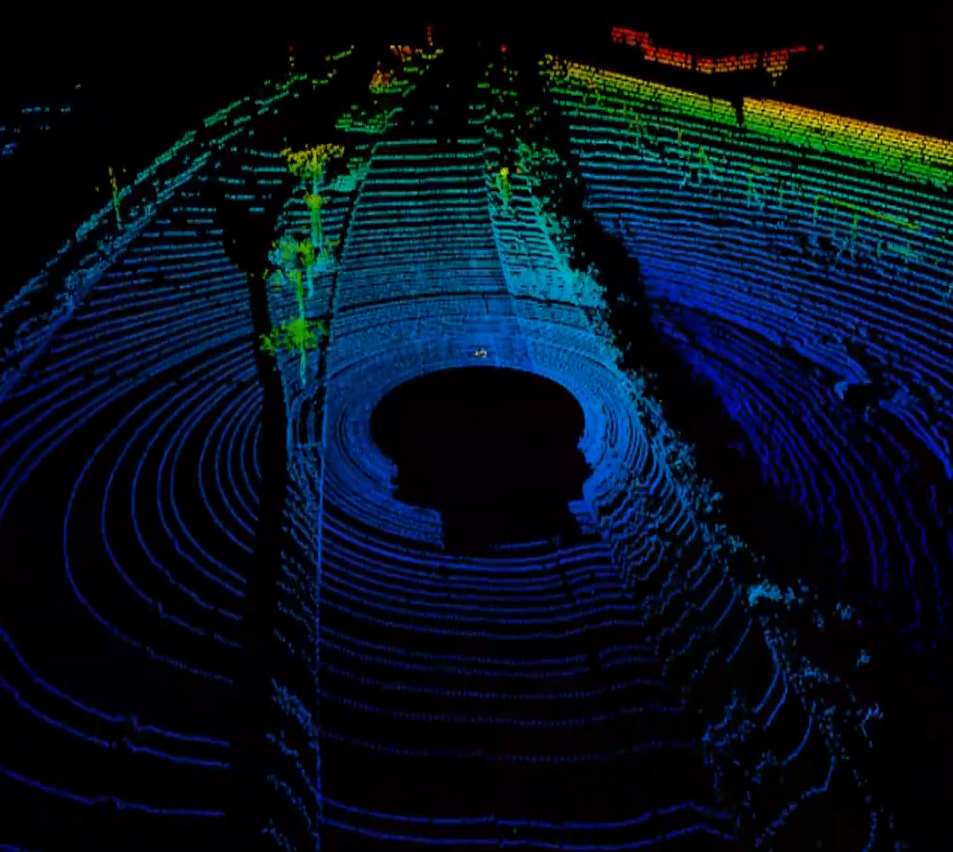
\includegraphics[height=0.32\textwidth]{fig/velodyne_scan.png}}
	\quad
	\subfloat[Robot vybavený senzormi]{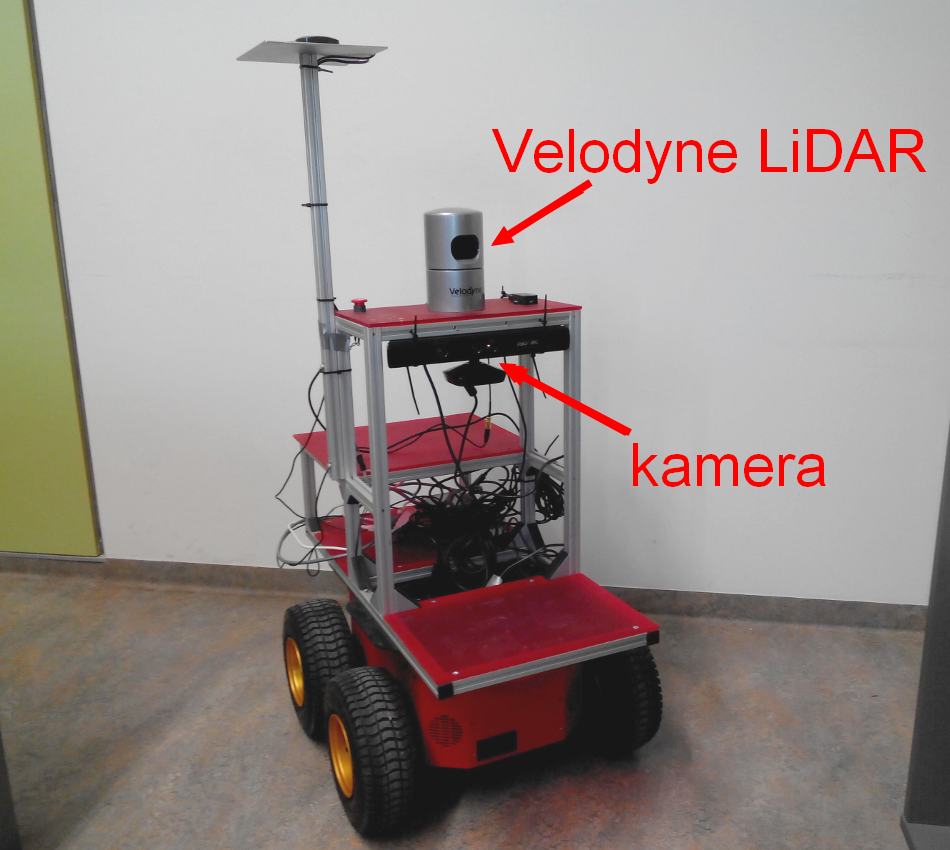
\includegraphics[height=0.32\textwidth]{fig/robot.png}}
\caption{Senzor Velodyne, príklad mračna bodov, ktoré sú jeho výstupom a inštalácia senzorov na našej robotickej platforme.\cite{velodyne}\label{fig:velodyne}}
\end{figure}

Jednoduchšie prevedenie s $32$ lúčmi má vertikálny zorný uhol v rozsahu od $-30^{\circ}$ do $+10^{\circ}$ a jeden snímok scény obsahuje približne $70\,000$ bodov. Maximálny dosah senzoru je okolo $70m$ a bežná presnosť okolo $2$cm.

%%%%%%%%%%%%%%%%%%%%%%%%%%%%%%%%%%%%%%%%%%%%%%%%%%%%%%%%%%%%%%%%%%%%%%%%%%%%%%%%
\section{Registrácia mračna bodov a RGB obrazu}
Prvým krokom k fúzii viacerých sníkov je ich registrácia -- t.j. určenie správneho zarovnania jedného snímku k druhému\cite{jan}. Tá je realizovaná pomocou výpočtu geometrickej transformácie medzi senzormi. V prípade viacerých senzorov je možné hovoriť o ich \emph{kalibrácii}.

Pre overenie správnosti geometrickej transformácie je nutné ďalej definovať vhodné kritérium podobnosti, založené na určitej spoločnej vlastnosti, ktorú zdieľa obraz a snímok LiDARu. Toto kritérium je možné ďalej využiť pri hľadaní samotnej geometrickej transformácie pomocou riešenia optimalizačnej úlohy.

\subsection{Geometrické transformácie}
Bez toho, aby boli zavedené dodatočné priestorové obmedzenia, je potrebné pri kalibrácii počítať so všetkými šiestimi stupňami voľnosti \emph{(6DoF, Degrees of Freedom)}\cite{taylor}. Teda s posunom jedného senzoru voči druhému v smere osi $x, y$ a $z$ a taktiež s rotáciou okolo týchto osí \emph{(pitch, roll, yaw)}.

Pri zavedení \emph{homogénnych súradníc} je každý $3$D bod $[x, y, z]$ reprezentovaný pomocou vektoru $[X, Y, Z, w]$ pričom platí, že
\begin{eqnarray}
	x &= \dfrac{X}{w} \\
	y &= \dfrac{Y}{w} \\
	z &= \dfrac{Z}{w}.
\end{eqnarray}

Posun (transláciu) a rotáciu určenú kalibračným procesom je potom možné reprezentovať pomocou \emph{kalibračnej matice} $C$, zloženej z koeficientov reprezentujúcich rotáciu $r_{i}$ a posun $t_j$. 

\begin{equation}
    C = \left[ 
      \begin{array}{cccc} 
	r_1 & r_2 & r_3 & t_1 \\
	r_4 & r_5 & r_6 & t_2 \\ 
	r_7 & r_8 & r_9 & t_3 \\
	0 & 0 & 0 & 1
      \end{array}  
      \right] \label{eq:translation}
\end{equation}

Posun a rotácia ľubovoľného bodu zo súradníc LiDARu $X_{lid}$ do bodu v súradniciach kamery $X_{cam}$ je realizovateľné jednoduchým maticovým násobením:

\begin{equation}
	X_{cam} = C . X_{lid}^T
\end{equation}

Keďže ide o fúziu $2$D snímkov s $3$D mračnom bodov, kalibrovaný snímok LiDARu je naviac premietnutý na rovinu obrazu pomocou projekčnej matice $P$, ktorá je odvodená na základe parametrov kamery -- \emph{ohnisková vzdialenosť} $f$ a \emph{principal point} $[o_x, o_y]$. Tento priemet je potom ďalej možné porovnať so snímkom kamery a tým overiť správnosť kalibrácie.

\begin{equation}
P = \left[ 
      \begin{array}{cccc} 
	f & 0 & o_x & 0 \\
	0 & f & o_y & 0 \\ 
	0 & 0 & 0 & 1
      \end{array}
    \right]	\label{eq:projection}
\end{equation}

Priemet $3$D bodu v (homogénnych) súradniciach kamery $X_{cam}$ na $2$D bod v štandardných súradniciach $[x, y]$ je možné potom opäť relizovať maticovým násobením a normalizáciou:

\begin{eqnarray}
	[X,Y,w] =& P . X_{cam}^T \\
	x =& \dfrac{X}{w} \\
	y =& \dfrac{Y}{w}
\end{eqnarray}

Opačný postup -- teda doplnenie hĺbkovej informácie do obrazu by bol možný napríklad pri použití stereo-obrazu. Nepresnosti odhadu hĺbkovej informácie a problémy pri zarovnávaní, ktorými sa vyznačujú mračná bodov Velodyne, tento postup však znemožňujú. 

\subsection{Projekčná chyba}
Pre hodnotenie kalibrácie boli v poslednej dobe navrhnuté viaceré techniky založené na detekcii hrán v obraze s využitím kroskorelácie \cite{levinson} alebo vzájomnej informácie \cite{taylor}. Vyhodnotenie publikované v \cite{velas} ukazuje, že uvedené kritériá vykazujú neobjektívne hodnotenie kalibrácie -- nepresná kalibrácie je ohodnotená vysokou hodnotou.

Tento problém je odstránený pri použití kritéria \emph{projekčnej chyby}, ktoré sa ukazuje ako objektívne hodnotenie vypočítanej kalibrácie. Vychádza z predpokladu, že body jednotlivých objektov v mračne bodov by mali byť premietnuté pri použití korektnej kalibračnej a projekčnej matice na oblasti obrazu, ktoré týmto objektom prináležia.

Výpočet tohto kritéria si vyžaduje zachytenie takej scény, pri ktorej bude možné spoľahlivo oddeliť -- \emph{segmentovať} -- oblasti jednotlivých objektov, prípadne oddelenie popredia od pozadia. Túto požiadavku spĺňa napríklad scéna zostavená pre potreby približnej hrubej kalibrácie, ktorá je vypočítaná na základe detekcie $3$D markeru (obr. \ref{fig:segmentation_scene}), ktorý je postavený pred iný kontrastný objekt (biela stena a pod.). Parametre tejto hrubej kalibrácie budú použité pre inicializáciu optimalizačnej úlohy, ktorá ju spresní.

V snímkoch takto pripravenej scény je možné segmentovať popredie od pozadia v obraze kamery pomocou \emph{adaptívneho prahovania} (výstup na obr. \ref{fig:segmentation_image}). Popredie (obr. \ref{fig:segmentation_front}) je možné oddeliť od pozadia (obr. \ref{fig:segmentation_back}) taktiež v mračne bodov zachytenom LiDARom segmentáciou pomocou metódy \emph{k-means}. V tomto prípade budú body popredia a pozadia predstavovať dva zhluky, ktoré sa táto metóda snaží nájsť.

\begin{figure}[h]
\center
	\subfloat[Pripravena scena]{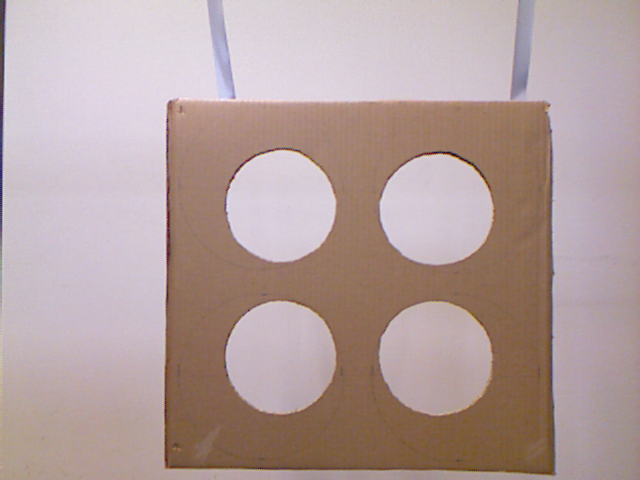
\includegraphics[height=0.25\textwidth]{fig/camera_left.png}\label{fig:segmentation_scene}}
	\quad
	\subfloat[Segmentacia obrazu]{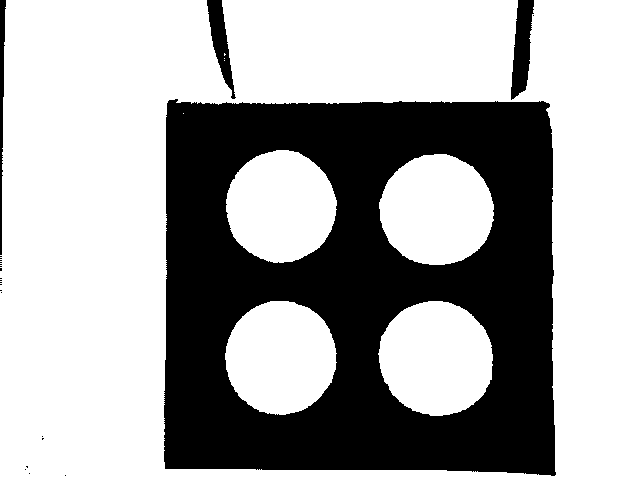
\includegraphics[height=0.25\textwidth]{fig/segment.png}\label{fig:segmentation_image}}
	
	\subfloat[Popredie mračna bodov]{
\includegraphics[height=0.3\textwidth]{fig/segment_front.png}\label{fig:segmentation_front}}
	\quad
	\subfloat[Pozadie mračna bodov]{
\includegraphics[height=0.3\textwidth]{fig/segment_back.png}\label{fig:segmentation_back}}
	
	\caption{Pripravená scéna pre výpočet projection error \protect\subref{fig:segmentation_scene}, segmenácia obrazu z kamery \protect\subref{fig:segmentation_image}, popredie \protect\subref{fig:segmentation_front} a pozadie \protect\subref{fig:segmentation_back} získamé segmentáciou mračna bodov.\label{fig:segmentation}}
\end{figure}

Výpočet projekčnej chyby je potom veľmi jednoduchý a priamočiary. Všetky body mračna sú premietnuté na rovinu obrazu pomocou vypočítanej kalibračnej a projekčnej matice, ako bolo uvedené v rovniciach \ref{eq:translation} a \ref{eq:projection}. Ak je bod popredia (mračno na obr. \ref{fig:segmentation_front}) premietnutý na segment popredia v obraze (čierny segment na obr. \ref{fig:segmentation_image}) alebo bod pozadia (obr. \ref{fig:segmentation_back}) na segment pozadia (biely segment na obr. \ref{fig:segmentation_image}), je táto projekcia úspešná. V opačnom prípade je bod prehlásený za nesprávne premietnutý. Projekčná chyba $E_P$ je potom určená ako
\begin{equation}
	E_P = \dfrac{P_{err}}{P_{all}},
\end{equation}

kde $P_{all}$ je celkový počet bodov v $3$D mračne a $P_{err}$ je počet neúspešne premietnutých bodov.

%%%%%%%%%%%%%%%%%%%%%%%%%%%%%%%%%%%%%%%%%%%%%%%%%%%%%%%%%%%%%%%%%%%%%%%%%%%%%%%%
\section{Optimalizácia kalibrácie pomocou evolučnej stratégie}

Na základe uvedených prístupov pre hodnotenie kalibrácie nie je možné matematicky odvodiť postup pre priamy výpočet geometrickej transformácie, ktorá je potrebná pre registráciu snímkov z kamery a LiDARu \cite{jan}. Úlohu kalibrácie je ale možné považovať za optimalizačný problém, pri ktorom je optimalizačné kritérium dané práve jedným z uvedených kritérií podobnosti -- v našom prípade pôjde o minimalizáciu projekčnej chyby $E_P$, resp. o maximalizáciu hodnoty $(1-E_P)$, keďže $E_P \in (0,1)$.

Na obrázku \ref{fig:nmi} je uvedený priebeh hodnotiacej funkcie kalibrácie založenej na detekcii hrán a výpočte vzájomnej informácie -- v tomto prípade je závislej na uhle rotácie medzi senzormi v smere dvoch osí. Je evidentné, že priebeh obsahuje veľa lokálnych optím. Táto vlastnosť hodnotiacej funkcie znemožňuje použitie typických prístupov k optimalizácii (znižovanie/zvyšovanie gradientu či Newtonovú optimalizáciu) \cite{jan}.

\begin{figure}[h]
\center
	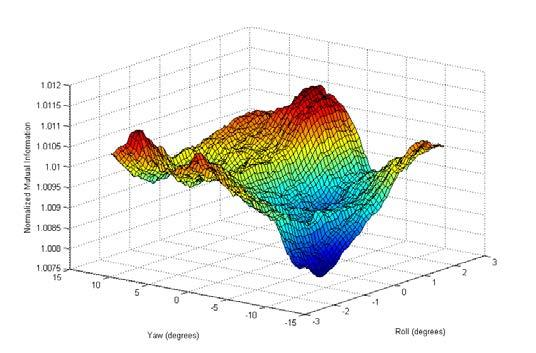
\includegraphics[width=0.6\textwidth]{fig/nmi_values.jpg}
\caption{Rozloženie normalizovanej vzájomnej informácie pri meniacom natočení podľa $x$-ovej a $y$-ovej osi.\cite{taylor}\label{fig:nmi}}
\end{figure}

Ideálnym prístupom by bolo úplné (resp. husté) prehľadávanie priestoru optimalizovaných parametrov. To však z dôvodu vysokej dimenzionality priestoru parametrov ($6$DoF) a jeho rozsahu nie je z výkonnostného hľadiska prípustné. Vhodným kompromisom sú techniky, ktoré kombinujú spomínané typické riešenia optimalizačných úloh so stochastickým prehľadávaním, ako napríklad optimalizácia evolučnou stratégiou.

Tento prístup je analogickým voči optimalizácii genetickým algoritmom, pri ktorom každý (binárny) vektor reprezentujúci riešenie považovaný za jedinca populácie \cite{kvasnicka}. Jedinci populácie vytvárajú nových potomkov pomocou operátorov kríženia a mutácie, ktoré realizujú samotné prehľadávanie priestoru parametrov a vnášajú do populácie diverzitu.

Ďalším prvkom genetického algoritmu a taktiež evolučnej stratégie je preferovanie silnejších jedincov -- s vyššou hodnotou fitnes, či už v procese výberu jedincov pre kríženie a teda aj tvorbu novej populácie (pri genetickom algoritme) alebo pri výbere jedincov do novej generácie populácie. 

Jednotlivé prvky evolučnej stratégie budú vysvetlené v nasledujúcich sekciách.

\subsection{Kódovanie problému}

Evolučná stratégia (napr. na rozdiel od genetických algoritmov) vyžaduje kódovanie problému vo forme vektoru reálnych čísel -- \emph{cieľových premenných}, ktorý vieme vyhodnotiť \emph{fitnes} funkciou v kontexte riešenej úlohy \cite{kvasnicka}.

V prípade kalibrácie kamery a LiDARu je cieľovými premennými $6$ stupňov voľnosti -- posun a natočenie LiDARu voči kamere vo všetkých $3$ osiach $3$D priestoru. Pre hodnotenie tohto vektoru bude použitá hodnota $(1-E_P)$ odvodená z projekčnej chyby $E_P$
\begin{equation}
	E_P: \mathcal{R}^6 \rightarrow (0,1),
\end{equation}
ktorá charakterizuje fitnes daného vektoru kalibračných parametrov, ktorý predstavuje jedného jedinca populácie.

\subsection{Stratégia (1+1)}

Pri tejto stratégii je populácia tvorená jediným jedincom, ktorý je v ďalšej generácii nahradený svojím potomkom získaným operátorom náhodnej \emph{mutácie} \cite{kvasnicka}. Ten ovplyvňuje aktuálne riešenie $\mathbf{x}$ malými zmenami s normálnym Gaussovým rozložením pravdepodobnosti so strednou hodnotou $\mu = 0$ a smerodajnou odchýlkou $\sigma$:
\begin{equation}
	\mathbf{x} := \mathbf{x} + N(0,\sigma)
\end{equation}

Priebeh jednočlennej evolučnej stratégie je popísaný algoritmom \ref{alg:evolution_single}. Vstupom tohto algoritmu je iniciálny vektor cieľových parametrov, interval vymedzujúci hodnoty, ktoré môžu cieľové parametre nadobúdať a smerodajnú odchýlku mutačného operátoru. Výstupom algoritmu je vektor cieľových parametrov s maximálnou hodnotou fitnes.

\begin{algorithm}[h]
	\dontprintsemicolon
	\KwIn{Iniciálny vektor reálnych premenných $x$, interval $(a,b)$ vymedzujúci možné hodnoty optimalizovaných parametrov a smerodajná odchýlka $\sigma_0$.}
	\KwOut{Vektor $x^*$ s najlepšou nájdenou fitnes.}
	\BlankLine
	
	$t$ := $0$\;
	$\sigma$ := $\sigma_0$\;
	$\mathbf{x^*}$ := $\mathbf{x}$\;	
	
	\While {$t < t_{max}$}
	{
		$i$ := $0$\;
		$k$ := $0$\;
		$t++$\;
		\While {$i < i_{max}$}
		{
			$i++$\;
			$\mathbf{x'}$ := $\mathbf{x} + \mathbf{N}(\mathbf{0}, \sigma)$\;
			\If { f($\mathbf{x'}$) < f($\mathbf{x}$) }
			{
				$k++$\;
				$\mathbf{x}$ := $\mathbf{x'}$\;
				\If { f($\mathbf{x}$) < f($\mathbf{x^*}$) }
				{
					$\mathbf{x^*}$ := $\mathbf{x}$\;	
				}
			}
			\If { $k/i_{max} < 0.2$ }
			{
				$\sigma$ := $c_d\sigma$\;
			} \ElseIf { $k/i_{max} > 0.2$ }
			{
				$\sigma$ := $c_i\sigma$\;
			}
		}
	}

	\Return{$\mathbf{x^*}$}
	\caption{\emph{Algoritmus evolučnej stratégie $(1+1)$} \cite{kvasnicka}\label{alg:evolution_single}}
\end{algorithm} 

Iniciálny vektor je možné vygenerovať náhodne rešpektujúc interval $(a,b)$. V prípade optimalizácie kalibrácie budú použité hodnoty cieľových parametrov poskytnuté predošlým procesom hrubého odhadu, ktorý je bližšie popísaný v predošlej publikácii \cite{velas}.

Počas priebehu výpočtu evolučnej stratégie je potrebné  zabezpečiť, aby mutované hodnoty cieľových parametrov hodnotou $n \sim N(0,\sigma)$ zostávali v intervale $(a,b)$ pomocou tzv. \emph{odrazu} popísaného vzťahom \ref{eq:pertrub1} a \ref{eq:pertrub2}, ktorý hodnotu parametru $x$ vráti do žiadaného intervalu.
\begin{eqnarray}
	x_n :=& x + n \label{eq:pertrub1}\\
	x :=& \left\{ \begin{array}{lcl}
	x_n      &    & x_n \in (a,b) \\
	2a - x_n & ak & x_n < a \\
	2b - x_n &    & x_n > b \\
	\end{array}\right.\label{eq:pertrub2}
\end{eqnarray}

Hodnota smerodajnej odchýlky môže podliehať v priebehu výpočtu taktiež zmenám. V prípade častých úspešne nájdených lepších riešení je hodnota $\sigma$ zväčšovaná násobením vhodnou konštantou $c_i = 1.22$ aby sa miera mutačných zmien podporila. Pri opačnom trende je smerodajná odchýlka násobená jej inverznou hodnotou $c_d = 1/c_i$ pre spomalenie mutačných zmien, ktoré aktuálne neprinášajú časté zlepšenie riešenia.

\subsection{Mnohočlenná stratégia (m+l)}

Pri použití tejto stratégie výpočet založený na použití viacerých  -- $m$ -- jedincov populácie, ktorí pomocou operátorov kríženia a mutácie vytvárajú v každej generácii $l$ nových potomkov \cite{kvasnicka}. Z tejto množiny jedincov ($m$ rodičov a $l$ potomkov) je vybraných $m$ jedincov s najlepšou fitnes, ktorí budú tvoriť populáciu ďalšej generácie výpočtu. Pre úlohy, ktorým hrozí uviaznutie v lokálnom minime je vhodný pomer $m:l = 1:7$.

Algoritmus \ref{alg:evolution_multiple} demonštruje postup výpočtu mnohočlennej evolučnej stratégie, ktorej výstupom je opäť jedinec s najlepšou nájdenou hodnotou fitnes.

\begin{algorithm}[h]
	\dontprintsemicolon
	\KwIn{interval $(a,b)$ vymedzujúci možné hodnoty optimalizovaných parametrov.}
	\KwOut{Vektor s najlepšou nájdenou fitnes.}
	\BlankLine
	
	$t$ := $0$\;
	$\sigma$ := $\sigma_{ini}$\;
	$P_0$ := \{náhodne generovaná populácia chromozómov (alely z intervalu $(a,b)$)\}\;
	
	\While {$t < t_{max}$ \textbf{alebo} nájdený chromozóm s dostatočnou fitnes }
	{
		$t++$\;
		$Q$ := \{nové chromozómy vytvorené krížením a mutáciou chromozómov $P_t$\}\;
		ohodnoť každý chromozóm $\mathbf{x}$ z $O$ hodnotou fitnes $f(\mathbf{x})$\;
		$P_t$ := \{najlepšie chromozómy z $Q \cup P_t$\}\;
	}

	\Return{$\underset{\mathbf{x}} {\mathrm{argmax}} \{f(\mathbf{x}) \vert \mathbf{x} \in P_t\}$}
	\caption{\emph{Algoritmus evolučnej stratégie $(1+1)$} \cite{kvasnicka}\label{alg:evolution_multiple}}
\end{algorithm} 

\subsubsection{Operátor kríženia}
Kríženie chromozómov populácie je ďalší spôsob (popri mutácii), ako je do populácie vnášaná rozmanitosť -- diverzita. Kríženie je použité už v oblasti genetických algoritmov, kde výmenou informácií dvoch jedincov vznikajú dvaja potomkovia. V prípade mnohočlenných evolučných stratégií je však výstupom kríženia jediný jedinec.

Prvým problémom, ktorý je pri zavedení kríženia potrebné vyriešiť je výber rodičovských jedincov, ktorý sa pre kríženie použijú. Evolučné stratégie vychádzaj z predpokladu, že konvergencia riešenia je zabezpečená selekciou najsilnejších jedincov do novej generácie a preto výber rodičov pre tvorbu novej populácie nereflektuje if fitnes (ako je to u genetických algoritmov), ale rodičia sú vyberaní s rovnomerných rozložením pravdepodobnosti.

Základné typy kríženia pri použití reálnych parametrov sú \emph{diskrétne kríženie}, ktoré vnáša najväčšiu mieru rozmanitosti do populácie. Ďalej kríženie \emph{priemerom} a \emph{lineárnou kombináciou}.

Pri diskrétnom krížení je každý cieľový parameter potomka priamo prebraný od jedného z dvoch rodičov, pričom výber konkrétneho rodiča pre konkrétny $i$-ty parameter podlieha opäť rovnomernému rozloženiu pravdepodobnosti:
\begin{equation}
	x_i = x_i^{rodic1} \;\;\; \mbox{alebo} \;\;\; x_i^{rodic2}.
\end{equation}

Kríženie priemerom realizuje bežný aritmetický priemer rodičovských vektorov:
\begin{equation}
	\mathbf{x} = \dfrac{\mathbf{x}^{rodic1} + \mathbf{x}^{rodic2}}{2}
\end{equation}

a posledný typ realizuje lineárnu kombináciu rodičov s koeficientom $\alpha$:
\begin{equation}
	\mathbf{x} = \mathbf{x}^{rodic1}\alpha + \mathbf{x}^{rodic2}(1-\alpha)
\end{equation}

\subsubsection{Evolúcia riadiacich parametrov}
Pri mnohočlennej evolučnej stratégii je na všetkých jedincov populácie (rodičov a potomkov) ďalej aplikovaný operátor mutácie rovnako, ako pri stratégii $(1+1)$. Riadiaci parameter $\sigma$ však nie je modifikovaný pravidlom $1/5$ ale každý jedinec obsahuje sadu riadiacich parametrov ${\sigma_i | i = 1 ... N}$ -- jeden pre každý z $N$ cieľových parametrov.

Tieto riadiace parametre -- smerodajné odchýlky podliehajú opäť evolučnej stratégií a sú mutované podľa vzťahu:
\begin{equation}
	\sigma_i := \sigma_i\exp^{N(0, \delta\sigma)}
\end{equation}

pričom hodnota $\delta\sigma$ je vstupným parametrom metódy a zostáva konštantná počas celého priebehu výpočtu evolučnej stratégie.

\section{Implementácia a vyhodnotenie}

Implementácia evolučnej stratégie $(1+1)$ a mnohočlennej stratégie vychádza z popisu metód uvedených v predchádzajúcej kapitole. Aplikácia je vytvorená s využitím knižnice počítačového videnia \emph{OpenCV}, knižnice pre prácu s mračnami bodov \emph{PCL} a v natívnom jazyku uvedených knižníc, ktorým je \emph{C++}. Podporné moduly \texttt{Velodyne} a \texttt{Image} vznikli pri príprave predchádzajúcej publikácie \cite{velas}.

Aplikácia je realizovaná s jednoduchým CLI rozhraním, pričom vstupnými argumentami sú obraz a projekčná matica kamery, mračno bodov LiDARu Velodyne a iniciálne hodnoty približnej kalibrácie. Zdrojové kódy sú verejne dostupné v osobnom repozitári \emph{GitHub} na adrese: 

\texttt{https://github.com/martin-velas/but\_calibration\_evolution}.

\medskip
Evolučná stratégia $(1+1)$ je implementovaná funkciou \texttt{evolution1x1} s využitím pomocnej triedy \texttt{CalibrationSubspace}. Stratégia vychádza z algoritmu \ref{alg:evolution_single}, pričom úprava smerodajnej odchýlky pravidlom $1/5$ bola z implementácie vypustená, pretože prinášala nevhodné uviaznutia riešenia v lokálnych minimách.

Mnohočlenná stratégia $(m+l)$ vychádza taktiež plne z popisu uvedenom v predchádzajúcej kapitole (algoritmus \ref{alg:evolution_multiple}). Pre vytváranie nových jedincov bol použitý operátor diskrétneho kríženia a veľkosť populácie bola zvolená na základe experimentov ako $(m,l) = (100,700)$.

Prepínanie medzi použitím jednočlennej a mnohočlennej evolučnej stratégie je riešené pomocou definície makra \texttt{MULTIMEMBER\_EVOLUTION} na úrovni preprocesoru prekladača jazyka C++.

\subsection{Dosiahnuté výsledky}
Okrem experimentov pre nájdenie vhodných parametrov evolučnej stratégie boli vykonané experimenty s optimálnymi parametrami -- vždy $10$ behov -- uvedené sú priemerné a najlepšie dosiahnuté výsledky na dátovej sade získanej z robotickej platformy. Tieto experimenty sa zameriavajú na porovnanie kalibrácie pomocou evolučnej stratégie s pravidelným vzorkovaním podpriestoru kalibračných parametrov, ktoré bolo použité v predchádzajúcej práci. 

Pre všetky typy porovnávaných kalibrácií (jednočlenná, mnohočlenná stratégia a pravidelné prehľadávanie priestoru) bol priestor kalibračných parametrov obmedzený na posun LiDARu voči kamere vo všetkých $3$ osiach na $2cm$ a zmena orientácie na $6^\circ$. Pri pravidelnom prehľadávaní bol podpriestor všetkých šiestich stupňov voľnosti vzorkovaný pre každú dimenziu $5x$, čo dohromady predstavuje prehľadanie $5^6 = 15\,625$ vektorov kalibračných parametrov, ktoré trvá na testovanej platforme (bežný NB) približne $55$s.

\begin{figure}[h]
\center
	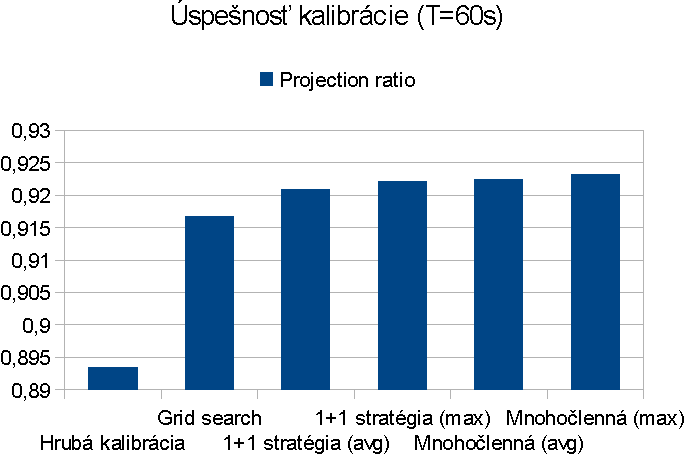
\includegraphics[width=0.8\textwidth]{fig/results.pdf}
\caption{Dosiahnutá fitnes $(1-E_P)$ iniciálnej kalibrácie, pravideľného prehľadávania priestoru, primerná a maximálna presnosť kalibrácie pri použití $(1+1)$ a mnohočlennej $(m+l)$ stratégie.\label{fig:results-accuracy}}
\end{figure}

V grafe na obr. \ref{fig:results-accuracy} sú uvedené hodnoty fitnes ($1-E_P$) pre jednotlivé testované prístupy ku kalibrácii, pričom každý z uvedených prístupov mal výpočetný čas obmedzený na $1$min. Z grafu vyplýva, že evolučná stratégia dosahuje mierne lepšie výsledky (obzvlášť mnohočlenná), ako jednoduché pravidelné vzorkovanie priestoru.

\begin{table}
	\center
	\begin{tabular}{|l|r|}
		\hline
		\textbf{Metóda} & \textbf{Čas [s]}\\
		\hline\hline
		Grid search & $55.0$ \\\hline
		Stratégia $(1+1)$ -- priemer & $3.9$ \\\hline
		Stratégia $(1+1)$ -- min     & $1.1$ \\\hline
		Stratégia $(m+l)$ -- priemer & $6.3$ \\\hline
		Stratégia $(m+l)$ -- min     & $3.6$ \\\hline
	\end{tabular}
	\caption{Porovnanie časovej náročnosti vyhľadania riešenia s porovnateľnou fitnes $(0.92)$.\label{tab:results-time}}
\end{table}

Výrazná zmena vo výkonnosti nastáva v prípade, že limitujúcim prvkom nie je výpočetný čas, ale snaha o dosiahnutie konkrétnej (resp. lepšej) hodnoty fitnes funkcie. V tomto prípade bola zvolená hodnota fitnes na hranicu $0.92$ (fitnes dosiahnuteľná pravidelným vzorkovaním). Z tabuľky \ref{tab:results-time} je evidentné, že evolučná stratégia dosahuje rapídne zrýchlenie -- cca. $8.7$x pre mnohočlennú a $15.3$x pre jednočlennú stratégiu.   

%%%%%%%%%%%%%%%%%%%%%%%%%%%%%%%%%%%%%%%%%%%%%%%%%%%%%%%%%%%%%%%%%%%%%%%%%%%%%%%%
\section{Záver}
V tejto práci boli predstavené techniky používané pre kalibráciu kamery a laserového radaru s využitím evolučných stratégií. V prvej časti bolo predstavené využitie takejto kalibrácie, prehľad senzorov a teoretický základ danej problematiky. Následne boli diskutované prístupy ku kalibrácii s využitím jednočlenných a mnohočlenných evolučných stratégií.

Podľa uvedených prístupov bola implementovaná aplikácia pre realizáciu kalibrácie jednočlennou a mnohočlennou evolučnou stratégiou. Na základe uvedených vykonaných experimentov bolo ukázané, že evolučné stratégie sú schopné poskytnúť lepšie výsledky kalibrácie a dokážu proces kalibrácie urýchliť až $15.3$x v porovnaní s naivným prístupom pravidelného vzorkovania podpriestoru kalibračných parametrov.

\bibliographystyle{czechiso}
\begin{flushleft}
  \bibliography{project}
\end{flushleft}

\end{document}
